\phantomsection
\section*{Chapter 3}
\addcontentsline{toc}{section}{Chapter 3}

\subsection*{3.6}

\begin{figure}[H]
  \centering
  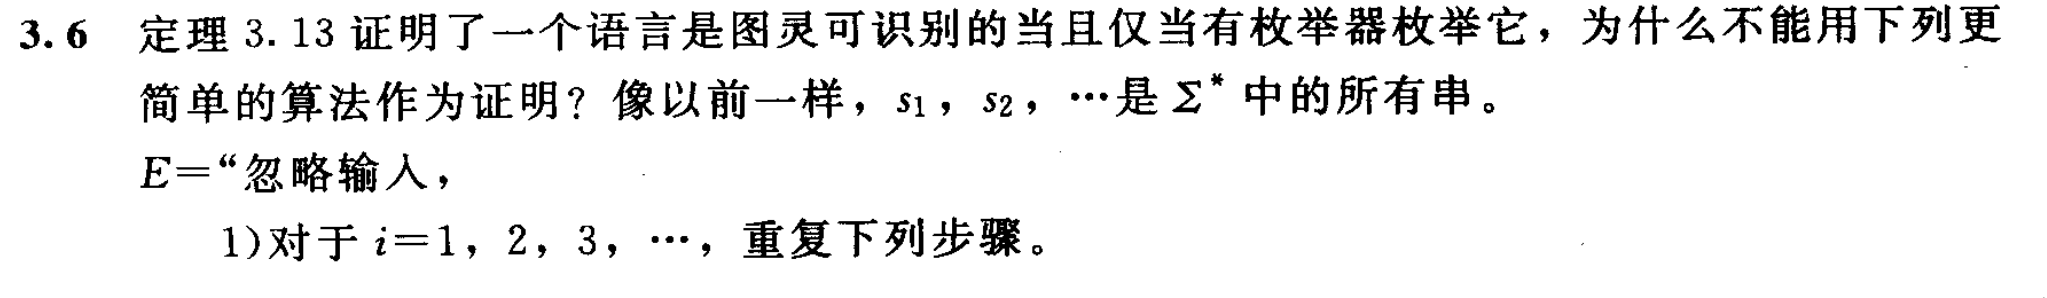
\includegraphics[width=\textwidth]{chapters/imgs/hw_3_6_p1.png}
  \caption{}
  \label{fig:hw_3_6_p1}
\end{figure}

\begin{figure}[H]
  \centering
  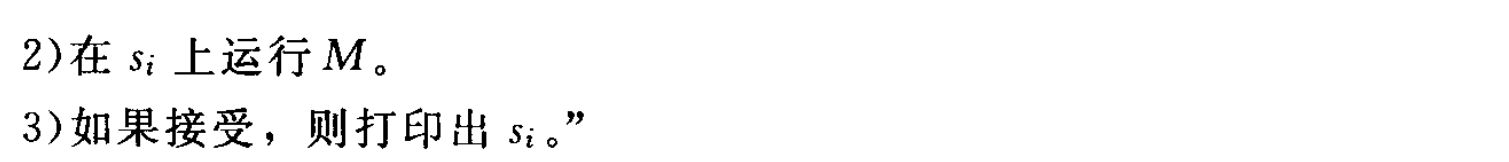
\includegraphics[width=\textwidth]{chapters/imgs/hw_3_6_p2.png}
  \caption{}
  \label{fig:hw_3_6_p2}
\end{figure}

证明。不能用题目中给出的更简单算法，是因为 $M$ 只是图灵可识别器，不一定对每个输入都停机。

若按题目中的方法枚举，到了某个字符串 $s_i$ 时，步骤 2 会在 $s_i$ 上一直运行 $M$。如果
\[
    M\text{ 在 }s_i\text{ 上循环而不停机},
\]
则枚举器就会永远卡在这一步，再也不会继续处理
\[
    s_{i+1},s_{i+2},\dots
\]

这样一来，即使后面某个字符串 $s_j$ 满足
\[
    s_j\in L(M),
\]
它也永远不会被打印出来。因此这个算法不能保证枚举出语言中的所有字符串。

这正是定理 3.13 正向证明里必须采用交错模拟（dovetailing）的原因：在第 $t$ 轮同时把前 $t$ 个输入都只模拟有限步，从而不会因为某一个输入上的无限循环而阻塞整个枚举过程。$\blacksquare$

\paragraph{解释.}
枚举器最怕“某个分支把全局卡死”。对图灵可识别器来说，某些输入上可能永远不停机，所以不能把全部时间都压在单个 $s_i$ 上；必须把时间公平地分给所有候选输入。

\subsection*{3.8}

\begin{figure}[H]
  \centering
  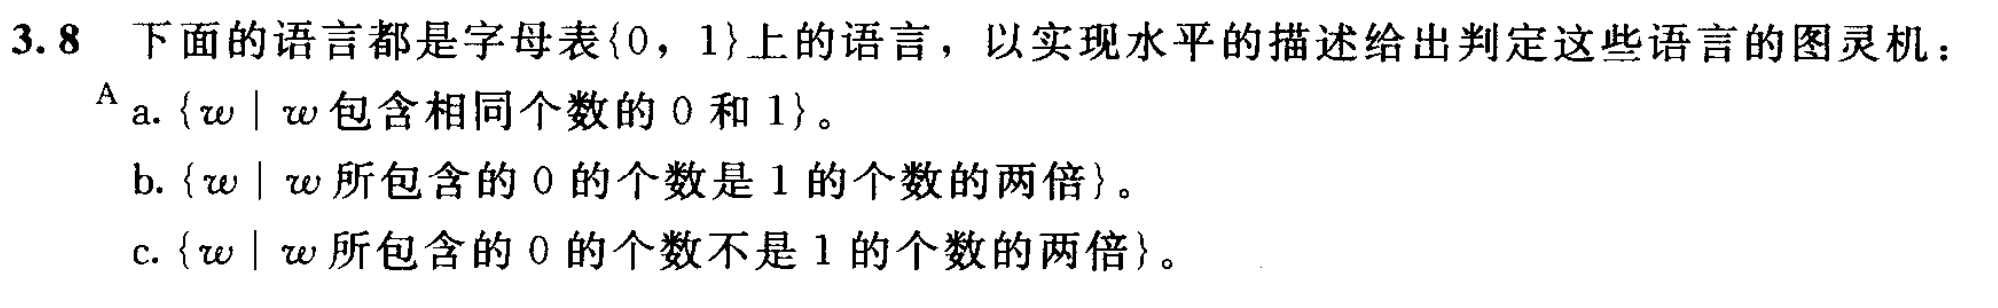
\includegraphics[width=\textwidth]{chapters/imgs/hw_3_8.png}
  \caption{}
  \label{fig:hw_3_8}
\end{figure}

设带字母表中另外加入标记符号 $X$，表示“这个位置已经配对过”。

\paragraph{(a)}
构造判定
\[
    A=\{w\mid w\text{ 中 }0\text{ 和 }1\text{ 的个数相同}\}
\]
的图灵机 $M_A$ 如下。

\medskip
\noindent
输入 $w$ 后：

\medskip
\noindent
1. 从带子左端开始向右扫描，找第一个尚未标记的符号。

\medskip
\noindent
2. 如果找不到这样的符号，说明所有 $0,1$ 都已成对删去，接受。

\medskip
\noindent
3. 若找到的是 $0$，就把它改写成 $X$，然后继续向右寻找第一个尚未标记的 $1$。若找不到，则拒绝；若找到，则把该 $1$ 也改写成 $X$。

\medskip
\noindent
4. 若找到的是 $1$，则对称地处理：把它改写成 $X$，再向右寻找第一个尚未标记的 $0$；若找不到则拒绝，若找到则也改写成 $X$。

\medskip
\noindent
5. 回到带子左端，重复上述过程。

\medskip
每一轮恰好删去一个 $0$ 和一个 $1$，因此机器必停机，并且当且仅当二者个数相等时接受。

\paragraph{(b)}
构造判定
\[
    B=\{w\mid w\text{ 中 }0\text{ 的个数是 }1\text{ 的个数的两倍}\}
\]
的图灵机 $M_B$ 如下。

\medskip
\noindent
1. 从左端开始寻找第一个尚未标记的 $1$。若不存在这样的 $1$，转第 4 步。

\medskip
\noindent
2. 把该 $1$ 改写成 $X$，然后从当前位置向右寻找两个尚未标记的 $0$。每找到一个就改写成 $X$。

\medskip
\noindent
3. 若在找满两个 $0$ 之前已无未标记的 $0$，则拒绝；否则回到左端继续第 1 步。

\medskip
\noindent
4. 此时所有 $1$ 都已处理完。再从左到右扫描一遍：若还存在未标记的 $0$，则拒绝；否则接受。

\medskip
每轮删去一个 $1$ 和两个 $0$，所以机器必停机，并且当且仅当
\[
    \#0=2\#1
\]
时接受。

\paragraph{(c)}
设
\[
    C=\{w\mid w\text{ 中 }0\text{ 的个数不是 }1\text{ 的个数的两倍}\}.
\]
因为 (b) 中的 $M_B$ 是 $B$ 的判定器，所以只需构造机器 $M_C$：

\medskip
\noindent
在输入 $w$ 上运行 $M_B$；若 $M_B$ 接受，则拒绝；若 $M_B$ 拒绝，则接受。

\medskip
于是 $M_C$ 判定 $C$。$\blacksquare$

\paragraph{解释.}
这三小题的核心都是“反复做有限次配对并标记”。(a) 是每次配走一个 $0$ 和一个 $1$；(b) 是每次配走两个 $0$ 和一个 $1$；(c) 直接利用 (b) 的补语言即可，因为 (b) 已经是判定器。

\subsection*{3.10}

\begin{figure}[H]
  \centering
  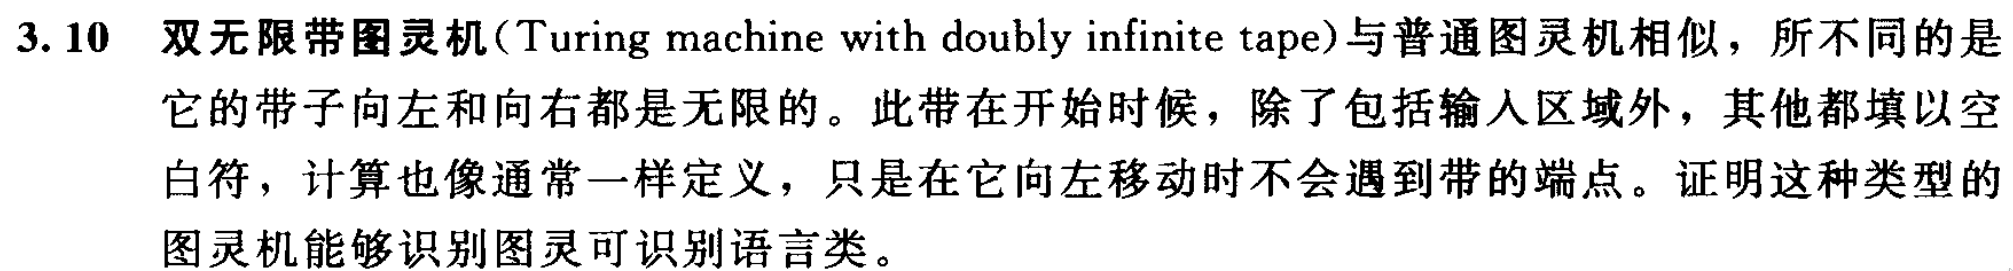
\includegraphics[width=\textwidth]{chapters/imgs/hw_3_10.png}
  \caption{}
  \label{fig:hw_3_10}
\end{figure}

证明。设双无限带图灵机所识别的语言类为 $\mathcal C$，普通图灵机所识别的语言类为 $\mathcal R$。

\medskip
\noindent
先证
\[
    \mathcal R\subseteq \mathcal C.
\]

这是显然的：普通图灵机只是双无限带图灵机的一种特殊情形，只要从不使用输入左侧那些额外的格子即可。

\medskip
\noindent
再证
\[
    \mathcal C\subseteq \mathcal R.
\]

设 $D$ 是一台双无限带图灵机。构造一台普通图灵机 $M$ 来模拟它。

\medskip
把 $D$ 的带内容编码成
\[
    u\#v,
\]
其中：

\medskip
\noindent
1. $v$ 记录当前读写头所在格及其右边各格的内容，当前格放在 $v$ 的最左端；

\medskip
\noindent
2. $u$ 记录当前读写头左边各格的内容，但按“离头越近越靠左”的逆序存放。

\medskip
也就是说，若 $D$ 的带在当前配置下形如
\[
    \cdots a_{-2}a_{-1}\underline{a_0}a_1a_2\cdots,
\]
则 $M$ 在自己的带上存放
\[
    a_{-1}a_{-2}\cdots \# a_0a_1a_2\cdots
\]
并把 $D$ 的当前状态记在有限控制中。

\medskip
现在说明如何模拟 $D$ 的一步转移。

\medskip
\noindent
1. 若 $D$ 在当前格写入符号 $b$，则 $M$ 只需把 $v$ 的第一个符号改写为 $b$。

\medskip
\noindent
2. 若 $D$ 向右移动，则 $M$ 把 $v$ 的第一个符号删去并接到 $u$ 的最左端。若删去后 $v$ 为空，则补上一个空白符，表示新当前格原本为空白。

\medskip
\noindent
3. 若 $D$ 向左移动，则 $M$ 把 $u$ 的第一个符号取出并放到 $v$ 的最左端；若 $u$ 为空，则取出的符号视为空白符。

\medskip
因此，$M$ 用有限次普通图灵机操作就能模拟 $D$ 的一步。于是 $M$ 能逐步模拟 $D$ 的整个计算，并在且仅在 $D$ 接受时接受。

故
\[
    L(M)=L(D).
\]

因此
\[
    \mathcal C=\mathcal R,
\]
即双无限带图灵机识别的正是图灵可识别语言类。$\blacksquare$

\paragraph{解释.}
双无限带并没有增加本质能力，因为“头左边的内容”和“头右边的内容”都可以用一条普通带上的有限编码保存。真正重要的不是带子朝哪边无限，而是机器是否能进行任意长的有限控制和重写。

\subsection*{3.12}

\begin{figure}[H]
  \centering
  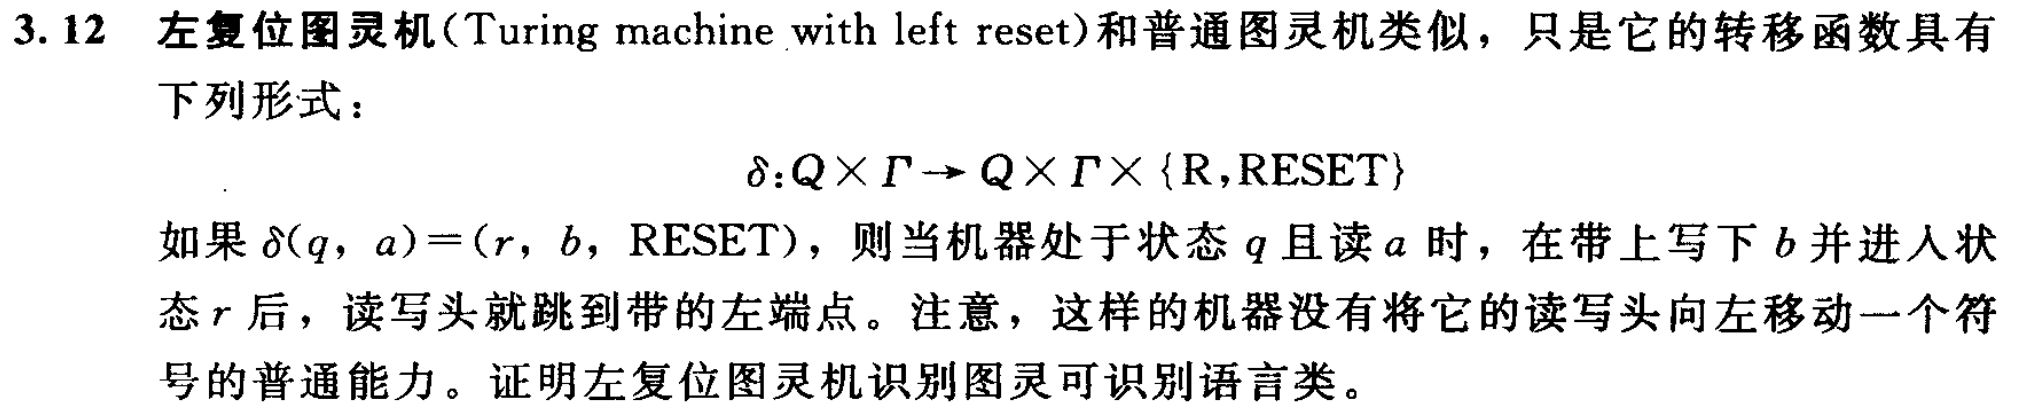
\includegraphics[width=\textwidth]{chapters/imgs/hw_3_12.png}
  \caption{}
  \label{fig:hw_3_12}
\end{figure}

证明。设左复位图灵机识别的语言类为 $\mathcal C$，普通图灵机识别的语言类为 $\mathcal R$。

\medskip
\noindent
先证
\[
    \mathcal C\subseteq \mathcal R.
\]

给定一台左复位图灵机，只需用普通图灵机来模拟其转移即可。对右移转移照常模拟；若遇到
\[
    \mathrm{RESET},
\]
就不断向左移动，直到到达带的左端点。这样普通图灵机即可逐步模拟左复位图灵机。

\medskip
\noindent
再证
\[
    \mathcal R\subseteq \mathcal C.
\]

设 $M$ 是一台普通图灵机。构造左复位图灵机 $P$ 来模拟它。

\medskip
$P$ 在自己的带上保存 $M$ 当前配置的编码
\[
    \#u\,q\,a\,v\#,
\]
其中 $u,v\in\Gamma^*$，$q$ 是 $M$ 的当前状态，$a$ 是当前读写头所读到的符号。也就是说，$u$ 是头左边的带内容，$a$ 是当前格，$v$ 是头右边的带内容。

\medskip
现在说明如何模拟 $M$ 的一步。

\medskip
\noindent
1. $P$ 先执行一次 $\mathrm{RESET}$，从左到右扫描当前编码，找到唯一的局部片段
\[
    q\,a.
\]
于是就知道
\[
    \delta_M(q,a)=(r,b,D).
\]

\medskip
\noindent
2. 接着 $P$ 再次 $\mathrm{RESET}$，并通过若干次“从左到右扫描旧编码，再把新编码写到右侧空白区域”的过程，构造下一配置的编码。

\medskip
\noindent
若 $D=R$，则把
\[
    \#u\,q\,a\,c\,v\#
\]
改成
\[
    \#u\,b\,r\,c\,v\#.
\]
若当前格右边没有已写出的符号，则把 $c$ 视为空白符。

\medskip
\noindent
若 $D=L$，则把
\[
    \#u'\,c\,q\,a\,v\#
\]
改成
\[
    \#u'\,r\,c\,b\,v\#.
\]
若当前格左边没有已写出的符号，则把 $c$ 视为空白符。

\medskip
\noindent
3. 新编码完成后，$P$ 忽略旧编码，继续在新编码上模拟下一步。

\medskip
因为每次模拟一步只需要有限次
\[
    \mathrm{RESET}
\]
和有限次从左到右的扫描，所以 $P$ 能逐步模拟 $M$ 的全部计算。因此
\[
    L(P)=L(M).
\]

故
\[
    \mathcal C=\mathcal R,
\]
即左复位图灵机识别的也是图灵可识别语言类。$\blacksquare$

\paragraph{解释.}
左复位看起来比“向左移动一格”弱很多，但它仍然足以模拟普通图灵机。原因是：虽然它不能原地左移，但它可以反复回到左端，再把整个当前配置重新扫描并重写成“下一配置”。代价只是时间变慢，而不是能力变弱。

\subsection*{3.15}


\begin{figure}[H]
  \centering
  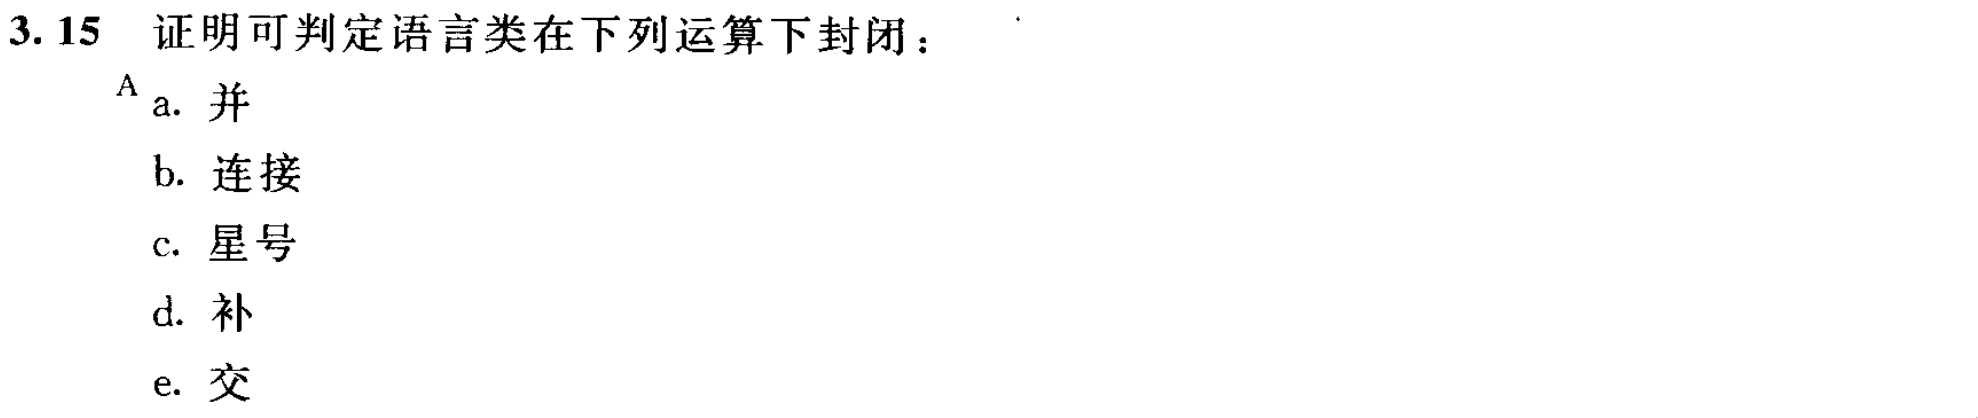
\includegraphics[width=\textwidth]{chapters/imgs/hw_3_15.png}
  \caption{}
  \label{fig:hw_3_15}
\end{figure}

设 $A,B$ 都是可判定语言，分别由判定器 $M_A,M_B$ 判定。

\paragraph{(a) 并}
构造判定器 $M$：

\medskip
\noindent
输入 $w$ 后，先运行 $M_A$ 于 $w$ 上。若 $M_A$ 接受，则接受；否则再运行 $M_B$ 于 $w$ 上。若 $M_B$ 接受，则接受；否则拒绝。

\medskip
因为 $M_A,M_B$ 都停机，所以 $M$ 停机，并且判定
\[
    A\cup B.
\]

\paragraph{(b) 连接}
构造判定器 $M$：

\medskip
\noindent
输入 $w$ 后，枚举所有分解
\[
    w=xy
\]
的方式。这样的分解只有 $|w|+1$ 种。对每一种分解，分别运行 $M_A$ 于 $x$ 上、$M_B$ 于 $y$ 上；若存在某种分解使得二者都接受，则接受；若所有分解都失败，则拒绝。

\medskip
因为分解数有限且每次调用都停机，所以 $M$ 判定
\[
    AB.
\]

\paragraph{(c) 星号}
构造判定器 $M$：

\medskip
\noindent
输入 $w$ 后，枚举把 $w$ 分割成有限多个子串
\[
    w=w_1w_2\cdots w_k
\]
的所有可能方式。若 $w=\varepsilon$，则直接接受。对每一种分割，逐个运行 $M_A$ 于各段 $w_i$ 上；若存在一种分割使得每一段都在 $A$ 中，则接受；若所有分割都失败，则拒绝。

\medskip
因为 $w$ 的分割方式只有有限多种，所以该机器停机，并判定
\[
    A^*.
\]

\paragraph{(d) 补}
构造判定器 $M$：

\medskip
\noindent
输入 $w$ 后运行 $M_A$。若 $M_A$ 接受，则拒绝；若 $M_A$ 拒绝，则接受。

\medskip
于是 $M$ 判定
\[
    \overline{A}.
\]

\paragraph{(e) 交}
构造判定器 $M$：

\medskip
\noindent
输入 $w$ 后，先运行 $M_A$，再运行 $M_B$。当且仅当二者都接受时接受，否则拒绝。

\medskip
因为 $M_A,M_B$ 都停机，所以 $M$ 判定
\[
    A\cap B.
\]

因此可判定语言类在并、连接、星号、补、交这五种运算下都封闭。$\blacksquare$

\paragraph{解释.}
证明“可判定”最关键的一点是：所有子过程都必须停机。并、交、补只是在已有判定器上做有限次组合；连接和星号虽然要“猜切分”，但输入长度固定时，切分方式只有有限种，所以也仍然能穷尽。

\subsection*{3.18}

\begin{figure}[H]
  \centering
  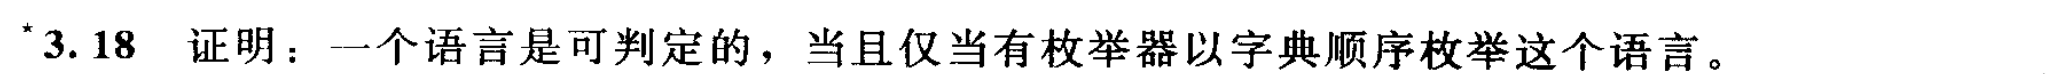
\includegraphics[width=\textwidth]{chapters/imgs/hw_3_18.png}
  \caption{}
  \label{fig:hw_3_18}
\end{figure}

证明。

\medskip
\noindent
先证“若 $A$ 可判定，则存在按字典顺序枚举 $A$ 的枚举器”。

\medskip
设 $M$ 是 $A$ 的判定器。构造枚举器 $E$：

\medskip
\noindent
忽略输入，按固定的字典顺序依次产生
\[
    s_1,s_2,s_3,\dots
\]
并对每个 $s_i$ 运行 $M$。若 $M$ 接受，则打印 $s_i$；若 $M$ 拒绝，则不打印，继续处理下一个字符串。

\medskip
因为 $M$ 对每个输入都停机，所以 $E$ 会依次检查所有字符串，并且恰好按字典顺序打印 $A$ 的所有成员。

\medskip
\noindent
再证“若存在按字典顺序枚举 $A$ 的枚举器，则 $A$ 可判定”。

\medskip
设 $E$ 按字典顺序枚举 $A$；若 $A$ 有限，则约定 $E$ 在输出最后一个字符串后停机。构造判定器 $D$：

\medskip
\noindent
输入字符串 $w$ 后，模拟 $E$ 的运行，并观察其打印输出。若 $E$ 打印出 $w$，则接受；若 $E$ 打印出某个严格大于 $w$ 的字符串，则拒绝；若 $E$ 在打印完所有不大于 $w$ 的字符串后停机，也拒绝。

\medskip
这个过程一定停机。因为在字典顺序中，不超过 $w$ 的字符串只有有限多个；而 $E$ 的输出又是递增的，所以最终只可能发生以下三种情况之一：

\medskip
\noindent
1. 打印出 $w$，此时 $w\in A$；

\medskip
\noindent
2. 先打印出一个严格大于 $w$ 的字符串，此时 $w\notin A$；

\medskip
\noindent
3. 输出完所有不大于 $w$ 的成员后停机，此时 $w\notin A$。

\medskip
因此 $D$ 判定 $A$。

综上，一个语言是可判定的，当且仅当存在枚举器按字典顺序枚举它。$\blacksquare$

\paragraph{解释.}
普通枚举器只能说明“可识别”，因为你不知道某个串只是“还没轮到”，还是“永远不会出现”。一旦输出顺序被限制成字典序，这种不确定性就消失了：只要已经越过了 $w$，就能立刻断定 $w\notin A$。

\subsection*{3.20}

\begin{figure}[H]
  \centering
  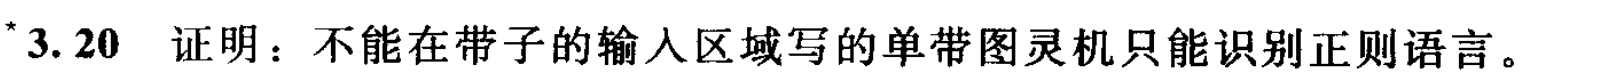
\includegraphics[width=\textwidth]{chapters/imgs/hw_3_20.png}
  \caption{}
  \label{fig:hw_3_20}
\end{figure}

证明。设 $M$ 是一台单带图灵机，并且它从不在初始输入所在的那一段区域内写符号。记它识别的语言为 $L(M)$。下面证明 $L(M)$ 必为正则语言。

\medskip
把带子分成两部分来看：

\medskip
\noindent
1. 左边是输入区域，内容从头到尾始终不变，因为 $M$ 不能在这里写入；

\medskip
\noindent
2. 右边是工作区域，$M$ 只能在那里改写。

\medskip
注意，一旦读写头离开输入区域进入工作区域，想要再次查看输入，就只能从输入的右端重新进入；而在它停留于输入区域期间，所见到的带内容完全固定，因此这段行为本质上就是一台\emph{双向有限自动机}在只读输入上的运行。

\medskip
更具体地说，对任意固定输入 $w$，以及任意状态 $q$，考虑如下“输入阶段”：

\medskip
\noindent
机器从输入右端进入只读输入区，起始状态为 $q$，随后一直在输入区内左右移动，直到发生以下三种情形之一：

\medskip
\noindent
1. 接受；

\medskip
\noindent
2. 拒绝；

\medskip
\noindent
3. 再次从输入右端离开，回到工作区，并以某个状态 $p$ 离开。

\medskip
由于输入区只读，这个“输入阶段”的结果只由
\[
    q\text{ 与 }w
\]
决定，而与工作区上存放了什么内容无关。于是，每个输入串 $w$ 都诱导出一个有限摘要：它告诉我们，对每个起始状态 $q$，上述输入阶段会得到哪一种结果。

\medskip
但是，输入区上的这种行为正是一台双向有限自动机对 $w$ 的行为。由 Rabin--Scott / Shepherdson 定理，双向有限自动机所识别的语言恰好是正则语言。因此，“给定一个有限摘要，哪些字符串产生这个摘要”构成正则语言。

\medskip
而整台机器 $M$ 对输入 $w$ 的判断，只能通过这些有限摘要来了解输入区的内容；工作区虽然可以保存任意多的信息，但它无法再从输入中获得超过该摘要之外的新信息。由于可能的摘要只有有限多个，$L(M)$ 只是其中若干个摘要类的并。

故
\[
    L(M)
\]
为正则语言。$\blacksquare$

\paragraph{解释.}
这题的核心限制不是“只有一条带”，而是“输入区永远不能被标记”。一旦不能在输入上留下记号，机器每次回到输入时，看到的仍然是同一个只读串；它对输入所能做的事情，本质上就退化成有限状态的双向扫描，而这种能力只对应正则语言。

\clearpage
